\documentclass[11pt,a4paper]{article}

\usepackage[margin=1in]{geometry}
\usepackage{times}
\usepackage{booktabs}
\usepackage{graphicx}
\usepackage{amsmath}
\usepackage{hyperref}
\usepackage{listings}
\usepackage{xcolor}
\usepackage{float}
\usepackage{tikz}
\usetikzlibrary{shapes.geometric, arrows.meta, positioning}

\hypersetup{
    colorlinks=true,
    linkcolor=blue,
    urlcolor=blue,
    citecolor=blue
}

\lstset{
    basicstyle=\small\ttfamily,
    breaklines=true,
    frame=single,
    backgroundcolor=\color{gray!10},
    keywordstyle=\color{blue},
    commentstyle=\color{green!50!black},
    stringstyle=\color{orange}
}

\title{\textbf{Building and Evaluating a Retrieval-Augmented Generation\\
System for LLM Course Q\&A}\\[0.5em]
\large COM SCI-X 450.46 Large Language Models --- Final Project (Track C)}

\author{JungleMist}
\date{June 2026}

\begin{document}

\maketitle

% ─────────────────────────────────────────────
\section{Introduction}
% ─────────────────────────────────────────────

Large Language Models (LLMs) have become increasingly capable of answering
natural-language questions, yet they still suffer from hallucination---generating
plausible but factually incorrect responses.  Retrieval-Augmented Generation
(RAG) addresses this by grounding the model's output in documents retrieved from
a curated knowledge base, rather than relying solely on memorised parameters.

This project implements and evaluates a complete RAG pipeline for answering
factual questions about the COM SCI-X 450.46 \emph{Large Language Models} course.
The corpus consists of syllabus materials, weekly overviews, and project
guidelines distributed throughout the course.  The system takes a natural-language
query, retrieves the most relevant text chunks from the indexed corpus using dense
embeddings, and generates an answer conditioned on those chunks.  Every answer is
then scored automatically using the RAGAS framework~\cite{ragas}, which measures
faithfulness, context precision, answer relevancy, and answer correctness against
human-written reference answers.

The central question is: \emph{to what extent can a RAG pipeline provide accurate,
faithful, and relevant answers to course-related queries, and where does it fail?}

% ─────────────────────────────────────────────
\section{Data \& Setup}
% ─────────────────────────────────────────────

\subsection{Document Corpus}

The knowledge base is built from the following course materials located in
\texttt{materials/}:

\begin{itemize}
    \item \textbf{LLM\_Syllabus.pdf} --- The official course syllabus (grading,
          schedule, textbook, project deliverables).
    \item \textbf{Week 1--8 Overview files} (\texttt{.md}) --- Per-week topic
          summaries covering all eight weeks of the course.
    \item \textbf{Final project guidelines} (\texttt{.md}) --- Proposal, prototype,
          peer-review, and final-submission rubrics.
    \item \textbf{LLM\_CoursePage.html} --- The public course page with enrolment
          and logistics information.
    \item \textbf{Hands-On Large Language Models} (textbook PDF) --- The required
          course text by Jay Alammar and Maarten Grootendorst.
\end{itemize}

In total the corpus spans 15 files comprising PDFs, Markdown files, and one HTML
page.  No external datasets were used; all documents are native course artefacts.

\subsection{Evaluation Dataset}

A hand-crafted evaluation set of \textbf{11 question--answer pairs}
(\texttt{dataset.json}) was constructed to cover the main topics in the corpus:
textbook information, project tracks and deliverables, weekly topics, prompting
strategies, RAG concepts, model optimisation techniques, and the distinction
between fine-tuning and zero-shot inference.  Reference answers were written to be
precise and factually grounded in the syllbus.

\subsection{Infrastructure}

\begin{itemize}
    \item \textbf{API endpoint (generation):} \texttt{https://ellm.nrp-nautilus.io/v1}
          (OpenAI-compatible), model \texttt{gpt-oss}, temperature 0.3.
    \item \textbf{Embedding model:} \texttt{qwen3-embedding} served via the same
          NRP endpoint.
    \item \textbf{Vector store:} ChromaDB (persistent, local).
    \item \textbf{Judge LLM (RAGAS):} DeepSeek via \texttt{https://api.deepseek.com},
          temperature 0 for determinism.
    \item \textbf{Chunking:} 400-character windows with 100-character overlap.
    \item \textbf{Retrieval top-$k$:} 3 chunks per query.
\end{itemize}

% ─────────────────────────────────────────────
\section{Methods}
% ─────────────────────────────────────────────

\subsection{System Architecture}

Figure~\ref{fig:pipeline} illustrates the end-to-end pipeline.

\begin{figure}[H]
\centering
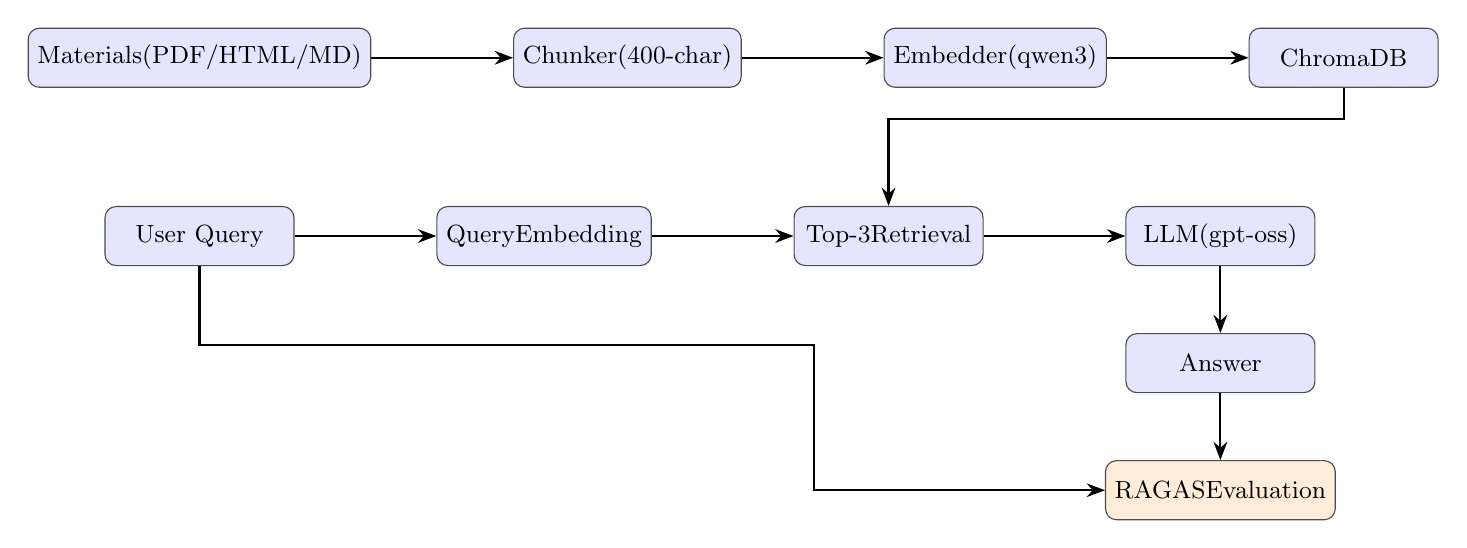
\begin{tikzpicture}[
    node distance=1.1cm and 1.8cm,
    box/.style={rectangle, rounded corners, draw=black!70, fill=blue!10,
                minimum width=2.4cm, minimum height=0.75cm,
                text centered, font=\small},
    arrow/.style={-Stealth, thick}
]

\node[box] (docs)    {Materials\\(PDF/HTML/MD)};
\node[box, right=of docs]  (chunk)   {Chunker\\(400-char)};
\node[box, right=of chunk] (embed)   {Embedder\\(qwen3)};
\node[box, right=of embed] (chroma)  {ChromaDB};

\node[box, below=1.5cm of docs] (query)  {User Query};
\node[box, right=of query] (qemb)    {Query\\Embedding};
\node[box, right=of qemb]  (ret)     {Top-3\\Retrieval};
\node[box, right=of ret]   (llm)     {LLM\\(gpt-oss)};
\node[box, below=0.85cm of llm] (ans) {Answer};

\node[box, below=0.85cm of ans, fill=orange!15] (ragas) {RAGAS\\Evaluation};

\draw[arrow] (docs)  -- (chunk);
\draw[arrow] (chunk) -- (embed);
\draw[arrow] (embed) -- (chroma);

\draw[arrow] (query) -- (qemb);
\draw[arrow] (qemb)  -- (ret);
\draw[arrow] (chroma.south) -- ++(0,-0.4) -| (ret.north);
\draw[arrow] (ret)   -- (llm);
\draw[arrow] (llm)   -- (ans);
\draw[arrow] (ans)   -- (ragas);
\draw[arrow] (query.south) -- ++(0,-1.0) -- ++(7.8,0) |- (ragas.west);

\end{tikzpicture}
\caption{RAG pipeline: documents are indexed offline (top row); queries trigger
         retrieval and generation at inference time (middle row); RAGAS scores are
         computed against reference answers (bottom).}
\label{fig:pipeline}
\end{figure}

\subsection{Document Loading and Chunking}

The \texttt{chunker.py} module handles three file types:

\begin{itemize}
    \item \textbf{PDF:} Page-by-page text extraction via \texttt{pypdf}.
    \item \textbf{HTML:} Full-document text stripped by \texttt{BeautifulSoup}.
    \item \textbf{Markdown/TXT:} Read directly as UTF-8 plaintext.
\end{itemize}

Documents are split into overlapping character-level windows
(chunk\_size = 400, overlap = 100).  Each chunk carries metadata
(\texttt{source}, \texttt{type}, \texttt{page}/\texttt{chunk\_index}).

\subsection{Incremental Indexing}

\texttt{indexer.py} maintains a \texttt{manifest.json} recording the SHA-256
hash of every indexed file.  On each run, only files whose hash has changed since
the previous run are re-embedded and upserted into ChromaDB
(\texttt{MiniRAG(force\_initial=False)}).  This avoids redundant API calls during
iterative development.

\subsection{Embedding and Retrieval}

Query and document embeddings are produced by \texttt{qwen3-embedding} via a
single \texttt{/embeddings} API call per text.  ChromaDB stores embeddings
persistently under \texttt{./chroma/}.  At query time, the nearest-3 chunks are
retrieved using L2 distance (lower = more similar).  Retrieved texts are
concatenated and injected into the system prompt via the
\texttt{prompts/retrieval.md} template:

\begin{lstlisting}[language={}]
You are a helpful course assistant. Please answer the question
from the user given the following contents.

**Relative contents**
{contents}
\end{lstlisting}

\subsection{Generation}

\texttt{llm/client.py} calls the NRP OpenAI-compatible endpoint with
\texttt{gpt-oss} at \texttt{temperature=0.3}.  A non-standard
\texttt{cache\_salt} header is passed in \texttt{extra\_body} to control
server-side caching specific to the NRP infrastructure.

\subsection{Automated Evaluation via RAGAS}

Every generated answer is scored by \texttt{llm/judge.py} using four RAGAS
metrics:

\begin{description}
    \item[Faithfulness] Fraction of answer claims that can be directly inferred
          from the retrieved context.  Computed by decomposing the answer into
          atomic claims and verifying each against the context via the judge LLM.
    \item[Context Precision] Whether the retrieved chunks are ranked such that the
          most relevant appear first; measures signal-to-noise in retrieval.
    \item[Answer Relevancy] Semantic similarity between the question and the
          generated answer (uses embeddings).  Penalises evasive or off-topic
          responses.
    \item[Answer Correctness] Weighted combination of semantic similarity and
          factual overlap between the generated answer and the reference answer.
\end{description}

All four metrics are computed concurrently with \texttt{asyncio.gather} to
reduce evaluation latency.

% ─────────────────────────────────────────────
\section{Experiments \& Results}
% ─────────────────────────────────────────────

\subsection{Evaluation Setup}

The full \texttt{dataset.json} (11 items) was processed by running
\texttt{main.py}, which executes the complete pipeline for each query and writes
results to \texttt{output.json}.

\subsection{Per-Query Results}

Table~\ref{tab:results} reports all four RAGAS scores for each query.

\begin{table}[H]
\centering
\small
\caption{RAGAS evaluation scores for all 11 queries (F = Faithfulness,
CP = Context Precision, AR = Answer Relevancy, AC = Answer Correctness).}
\label{tab:results}
\begin{tabular}{clcccc}
\toprule
\textbf{ID} & \textbf{Query (abbreviated)} & \textbf{F} & \textbf{CP} & \textbf{AR} & \textbf{AC} \\
\midrule
1  & Required textbook            & 0.00 & 0.00 & 0.978 & 0.218 \\
2  & Four project tracks          & 0.00 & 0.00 & 0.993 & 0.688 \\
3  & Week 3 topics                & 0.47 & 0.00 & 0.834 & 0.570 \\
4  & What is RAG, which week      & 0.63 & 1.00 & 0.970 & 0.593 \\
5  & Three prompting strategies   & 0.00 & 0.00 & 0.903 & 0.613 \\
6  & Required final project deliverables & 0.71 & 0.00 & 0.993 & 0.306 \\
7  & Week 8 optimisation techniques & 0.38 & 1.00 & 0.933 & 0.537 \\
8  & Evaluation topics and frameworks & 0.81 & 0.00 & 0.889 & 0.241 \\
9  & Python packages used         & 0.41 & 0.00 & 0.978 & 0.243 \\
10 & Fine-tuning vs.\ zero-shot   & 0.62 & 1.00 & 0.968 & 0.576 \\
11 & Project proposal requirements & 1.00 & 1.00 & 0.989 & 0.875 \\
\midrule
\textbf{Mean} & & \textbf{0.456} & \textbf{0.364} & \textbf{0.948} & \textbf{0.496} \\
\bottomrule
\end{tabular}
\end{table}

\subsection{Summary}

\begin{itemize}
    \item \textbf{Answer Relevancy} (mean 0.948) is consistently high, confirming
          the model produces responses that address the question being asked.
    \item \textbf{Answer Correctness} (mean 0.496) is moderate, indicating the
          generated content partially overlaps with reference answers but often
          contains extra or incorrect information.
    \item \textbf{Faithfulness} (mean 0.456) varies widely (0.00--1.00).  Low
          scores signal hallucination: the model asserts facts not present in the
          retrieved chunks.
    \item \textbf{Context Precision} (mean 0.364) is the weakest metric.  For
          most queries, the top-3 retrieved chunks do not place the most relevant
          content first, suggesting the embedding space or chunk boundaries do not
          align well with the query intent for many questions.
\end{itemize}

\subsection{With vs.\ Without Retrieval}

Table~\ref{tab:comparison} compares answer relevancy and answer correctness across
both conditions for all 11 queries.  Faithfulness and context precision are omitted
for the no-RAG condition because they require retrieved context by definition.

\begin{table}[H]
\centering
\small
\caption{Answer Relevancy (AR) and Answer Correctness (AC): RAG vs.\ no-RAG baseline.}
\label{tab:comparison}
\begin{tabular}{clcccc}
\toprule
& & \multicolumn{2}{c}{\textbf{RAG}} & \multicolumn{2}{c}{\textbf{No-RAG}} \\
\cmidrule(lr){3-4}\cmidrule(lr){5-6}
\textbf{ID} & \textbf{Query (abbreviated)} & \textbf{AR} & \textbf{AC} & \textbf{AR} & \textbf{AC} \\
\midrule
1  & Required textbook               & 0.978 & 0.218 & 0.984 & 0.247 \\
2  & Four project tracks             & 0.993 & 0.688 & 0.971 & 0.427 \\
3  & Week 3 topics                   & 0.834 & 0.570 & 0.909 & 0.236 \\
4  & What is RAG, which week         & 0.970 & 0.593 & 0.982 & 0.696 \\
5  & Three prompting strategies      & 0.903 & 0.613 & 0.891 & 0.511 \\
6  & Required project deliverables   & 0.993 & 0.306 & 0.980 & 0.288 \\
7  & Week 8 optimisation techniques  & 0.933 & 0.537 & 0.925 & 0.621 \\
8  & Evaluation topics               & 0.889 & 0.241 & 0.983 & 0.242 \\
9  & Python packages used            & 0.978 & 0.243 & 0.972 & 0.237 \\
10 & Fine-tuning vs.\ zero-shot      & 0.968 & 0.576 & 0.966 & 0.631 \\
11 & Project proposal requirements   & 0.989 & 0.875 & 0.902 & 0.426 \\
\midrule
\textbf{Mean} & & \textbf{0.948} & \textbf{0.496} & \textbf{0.951} & \textbf{0.415} \\
\bottomrule
\end{tabular}
\end{table}

Both conditions achieve nearly identical answer relevancy ($\approx$0.95), confirming
the LLM consistently addresses the question regardless of whether context is provided.
Answer correctness is higher with RAG (0.496 vs.\ 0.415), driven by queries requiring
precise course-specific facts (e.g., exact textbook title, official track names and
letters, specific due dates) where retrieval grounds the model in the correct document.

% ─────────────────────────────────────────────
\section{Qualitative Analysis \& Error Cases}
% ─────────────────────────────────────────────

\subsection{Strong Case: Project Proposal Requirements (ID 11)}

Query ID 11 received the highest scores across all four metrics
(F=1.00, CP=1.00, AR=0.99, AC=0.88).  The syllabus PDF contains a dedicated
section on proposal requirements, producing dense, relevant chunks.  The LLM
accurately reproduced all six required elements (track, title, task description,
planned models, data, evaluation plan, backup plan) and the correct due date
(Monday, May 18).  This shows the pipeline functions correctly when document
coverage is precise and query specificity is high.

\subsection{Retrieval Failure: Required Textbook (ID 1)}

Query ID 1 scored F=0.00, CP=0.00, AC=0.22.  The generated answer confidently
named \emph{Deep Learning} by Goodfellow, Bengio, and Courville as the required
textbook---a fabrication.  The actual required text is \emph{Hands-On Large
Language Models} by Alammar and Grootendorst.

The root cause is a retrieval failure: the textbook PDF itself was indexed but
the relevant title/ISBN information appears on pages not captured by the top-3
chunks for this query.  Because the retrieved context contained no textbook name,
the LLM fell back to parametric memory and hallucinated a plausible-but-wrong
answer.  This is a canonical RAG failure mode: retrieval precision determines
answer faithfulness.

\subsection{Partial Retrieval: Project Tracks (ID 2)}

Query ID 2 received F=0.00, CP=0.00 but AC=0.69.  The LLM invented four
plausible-sounding tracks (Chatbot, RAG, Fine-tuning, Prompt Engineering)
instead of the four official ones (A: LLM Application, B: Prompt Design, C: RAG,
D: Fine-tuning).  The semantic overlap between the generated and reference answers
is substantial (hence the higher AC), but the official naming and framing were
missed.  This shows that even semantically correct answers can reflect
hallucinated specifics when the retrieved context lacks the verbatim source.

\subsection{Mixed Success: RAG Definition (ID 4)}

Query ID 4 scored well (F=0.63, CP=1.00, AC=0.59).  Context precision reached
1.00, meaning the most relevant chunk was retrieved first.  The answer correctly
identified Week 5 and gave an accurate definition of RAG.  Faithfulness was below
1.0 because several elaborations in the answer go beyond what was stated in the
retrieved text, though the core facts remain correct.

% ─────────────────────────────────────────────
\section{Ethics \& Limitations}
% ─────────────────────────────────────────────

\paragraph{Privacy.}
All course materials used in this project are either publicly available or
distributed to enrolled students.  No personally identifiable student data is
processed.

\paragraph{Bias.}
The corpus is a single instructor's course materials.  The system reflects the
perspective and terminology of those documents.  Queries about topics not
covered in the materials may produce hallucinated responses that sound equally
authoritative.

\paragraph{Hallucination.}
As demonstrated by Query ID 1, the system can fabricate specific facts (book
titles, author names) when retrieval fails.  A production deployment would
require a confidence signal or a fallback ``I don't know'' response when
retrieved context is insufficient.

\paragraph{Evaluation Limitations.}
RAGAS metrics rely on a judge LLM (DeepSeek) that may itself be biased or
inconsistent.  The evaluation set of 11 items is small; a larger benchmark would
give more reliable estimates.  Context precision is particularly sensitive to
chunk boundary artifacts.

\paragraph{Scope.}
The chunker uses character-level splitting without sentence-boundary awareness.
This can cause mid-sentence cuts that degrade retrieval quality.  The system was
not tested against adversarial or out-of-domain queries.

% ─────────────────────────────────────────────
\section{Conclusion \& Future Work}
% ─────────────────────────────────────────────

This project built a working RAG pipeline for a domain-specific Q\&A task and
evaluated it with RAGAS.  The main findings are:

\begin{enumerate}
    \item Answer relevancy is consistently high ($\approx$0.95), confirming the
          pipeline produces on-topic responses.
    \item Faithfulness and context precision are the primary weaknesses, pointing
          to inadequate retrieval for specific factual queries.
    \item When the relevant text is indexed and retrieved correctly (as in ID 11),
          all four metrics are high, validating the overall architecture.
\end{enumerate}

\noindent \textbf{Key lesson:} In RAG systems, retrieval quality is the bottleneck.
A more capable embedding model, finer chunk granularity, or hybrid
keyword+semantic search would likely raise faithfulness and context precision
substantially.

\paragraph{Future work.}
\begin{itemize}
    \item \textbf{Sentence-aware chunking} --- split at sentence boundaries to avoid
          mid-sentence truncation.
    \item \textbf{Hybrid retrieval} --- combine BM25 keyword search with dense
          embeddings using Reciprocal Rank Fusion.
    \item \textbf{Larger evaluation set} --- expand \texttt{dataset.json} to 50+
          items for more reliable metric estimates.
    \item \textbf{Reranker} --- add a cross-encoder reranker to improve context
          precision before passing chunks to the LLM.
    \item \textbf{Confidence gating} --- detect low-relevance retrievals and return
          a fallback response rather than risk hallucination.
\end{itemize}

\begin{thebibliography}{9}
\bibitem{ragas}
    Shahul Es, Jithin James, Luis Espinosa-Anke, Steven Schockaert.
    \textit{RAGAS: Automated Evaluation of Retrieval Augmented Generation}.
    arXiv:2309.15217, 2023.

\bibitem{alammar}
    Jay Alammar, Maarten Grootendorst.
    \textit{Hands-On Large Language Models: Language Understanding and Generation}.
    O'Reilly Media, 2024. ISBN 1098150961.

\bibitem{chromadb}
    Jeff Huber, Anton Troynikov et al.
    \textit{Chroma: the AI-native open-source embedding database}.
    \url{https://www.trychroma.com}, 2023.

\bibitem{lewis2020rag}
    Patrick Lewis et al.
    \textit{Retrieval-Augmented Generation for Knowledge-Intensive NLP Tasks}.
    NeurIPS 2020.
\end{thebibliography}

\end{document}